\section{Introducción al Machine Learning}
\subsection*{¿Qué es el Machine Learning?}
\begin{itemize}[label=\color{red}\textbullet, leftmargin=*]
	\item \color{lightblue}Definición de Machine Learning
\end{itemize}
"Descubrir regularidades en datos mediante el uso de algoritmos, y mediante el uso de esas regularidades realizar alguna acción" (C. M. Bishop)
\begin{itemize}[label=\color{red}\textbullet, leftmargin=*]
	\item \color{lightblue}Tareas básicas
\end{itemize}
Fundamentalmente cuatro:
\begin{itemize}[label=\color{lightblue}\textbullet]
\item Clasificación
\begin{itemize}[label=\color{lightblue}$\to$]
\item \textbf{Detección de spam:} Se trata de clasificar, mediante identificación de patrones, los correos electrónicos como spam o no spam.
\item \textbf{Detección de fraudes:} Distinción entre transacciones legítimas y sospechosas basándose en patrones y características relevantes.
\item \textbf{Análisis de sentimientos:} Los algoritmos de clasificación pueden utilizarse para determinar el sentimiento expresado en un texto, como positivo, negativo o neutro. Esto es útil para el análisis de opiniones en redes sociales, comentarios de clientes, revisiones de productos, etc.
\item \textbf{Detección de objetos en imágenes:} Especialmente útil en la conducción de coches autónomos.
\end{itemize}
\item Regresión
\begin{itemize}[label=\color{lightblue}$\to$]
\item \textbf{Estimación de la demanda de un producto:} Predicción de la demanda de un producto en función de variables como el precio, la publicidad, las tendencias del mercado, entre otras.
\item \textbf{Predicción de la contaminación atmosférica:} Utilizando datos históricos de contaminantes, meteorología y otras variables relevantes, se puede aplicar la regresión para predecir los niveles de contaminación en una ubicación específica.
\item \textbf{Análisis de la relación entre variables económicas:} La regresión puede utilizarse para explorar la relación entre variables económicas, como el crecimiento del PIB y el desempleo, con el fin de entender mejor su interdependencia y tomar decisiones políticas o empresariales informadas.
\end{itemize}
\item Agrupamiento
\item Asociación
\end{itemize}
\begin{itemize}[label=\color{red}\textbullet, leftmargin=*]
	\item \color{lightblue}Tarea de agrupación en Machine Learning
\end{itemize}
El \textbf{agrupamiento} o \textbf{clustering} consiste en detectar agrupaciones en datos \underline{no etiquetados} empleando alguna media  de similitud entre ellas. El objetivo es descubrir patrones y estructuras dentro de los datos.

Algoritmos populares para clustering incluyen el K-Means, el DSCAN, el clustering jerárquico y Mapas Autoorganizados (SOM).

\bu{Ejemplo K-Means}
\begin{center}
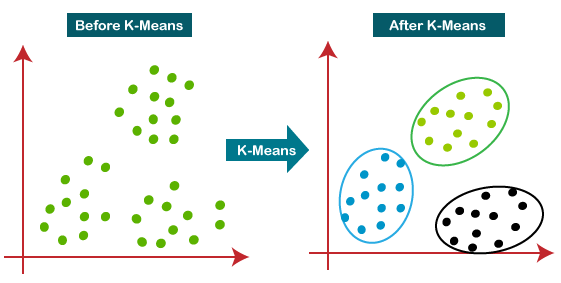
\includegraphics[scale=0.7]{"Temas/Tema 1/K-means.png"}
\end{center}
\begin{itemize}[label=\color{red}\textbullet, leftmargin=*]
	\item \color{lightblue}Tarea de asociación en Machine Learning
\end{itemize}

La tarea de \textbf{asociación} se centra en descubrir reglas de asociación entre eventos en un conjunto de datos, lo que significa identificar qué elementos tienden a aparecer juntos en dichos eventos. El objetivo es revelar después del afeitado, hay un 80\% de posibilidades de que el cliente compre también crema de afeitado.

La asociación es una tarea \underline{no supervisada}, los datos a menudo provienen de transacciones o eventos, y no se requieren etiquetas previas.

Algoritmos como Apriori se utilizan comúnmente para generar reglas de asociación en los datos, reglas como "Si A, entonces B". Estas reglas se utilizan en análisis de mercado y sistemas de recomendación.
\subsection{Planteamiento del problema}
En el contexto del Machine Learning, el \textbf{conjunto de hipótesis} se refiere a un conjunto de funciones o modelos matemáticos que se utilzian para aproximar una relación desconocida entre las \textbf{entradas $(x)$} y las \textbf{salidas deseadas o targets $(t)$} de un conjunto de datos.

Cada hipótesis representa una posible aproximación de la relación subyacente en los datos.

El objetivo del \textbf{aprendizaje supervisado} es encontrar la hipótesis que mejor se ajuste a los datos de entrenamiento manteniendo la capacidad de hacer predicciones precisas para datos nuevos \textbf{(capacidad de generalización)}.

\begin{center}
\begin{tikzpicture}
    % Define los nodos
    \node (A) at (0,0) {$x_j$};
    \node[draw=blue, right=2cm of A, text width=2cm, fill=lightblue!10] (B) {\begin{center}
    Máquina de \\ Aprendizaje \\ $y(x,w)$
    \end{center}};
    \node[right=2cm of B] (C) {$y(x_j,w)$};

    % Dibuja las flechas
    \draw[double -latex=4pt colored by lightblue and lightblue!10] (A) -- (B);
    \draw[double -latex=4pt colored by lightblue and lightblue!10] (B) -- (C);
\end{tikzpicture}
\end{center}

\begin{itemize}[label=\color{red}\textbullet, leftmargin=*]
	\item \lb{Necesario: Conjunto de entrenamiento}
	
	Pares: $\{x_j,t_j\}$ con $j=1,2,\dots,N$.\\
	$x_j=\{x_{j1},x_{j2},\dots,x_{jD}\}$ entrada $j$-ésima; vector con $D$ \textbf{componentes o características}.\\
	$t_j=\{x_{j1},x_{j2},\dots,x_{jT}\}$ target $j$-ésimo; vector con $T$ componentes.
	\item \lb{Objetivo: Aprendizaje supervisado}
	
	Encontrar las \textbf{variables o pesos} del modelo $(\mathbf{w})$ que resuelvan el problema: $y(x_j,\mathbf{w})\eqsim t_j$ para $j=1,2,\dots,N$. A esta tarea se la denomina \textbf{entrenamiento}.
\end{itemize}
\bu{Ejemplo: Problema de \textbf{regresión}}

$y=\sin(2\pi x)+n(x)$, donde $n(x)$ es un ruido gausiano pequeño.

\begin{wrapfigure}[3]{l}{0.3\textwidth}
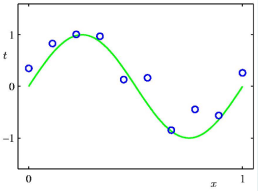
\includegraphics{"Temas/Tema 1/Entrenamiento.png"}
\end{wrapfigure}

Conjunto de entrenamiento: $\{x_j,t_j\}_{j=1}^{N=10}$

\begin{flushright}
\begin{tikzpicture}
    % Define los nodos
    \node (A) at (0,0) {$x_j$};
    \node[draw=blue, right=2cm of A, text width=2cm, fill=lightblue!10] (B) {\begin{center}
    Máquina de \\ Aprendizaje \\ $y(x,w)$
    \end{center}};
    \node[right=2cm of B] (C) {$y(x_j,w)$};

    % Dibuja las flechas
    \draw[double -latex=4pt colored by lightblue and lightblue!10] (A) -- (B);
    \draw[double -latex=4pt colored by lightblue and lightblue!10] (B) -- (C);
\end{tikzpicture}
\end{flushright}

Aproximador polinómico: $y(x,\mathbf{w})=w_0+w_1x+w_2x^2+\cdots+x_Mx^M=\sum_{j=0}^{M}x_jx^j$

\begin{itemize}
\item $M$ es un parámetro que determina la complejidad del modelo (orden del polinomio).
\item Los parámetros no entrenables que determinan el modelo o el entrenamiento se denominan en Machine Learning \textbf{hiperparámetros}.
\end{itemize}
\subsection{Planteamiento de la solución}
Se quiere encontrar las variables del modelos (coeficientes del polinomio) para que éste minimice una función de coste o error, por ejemplo, la función de error SSE ("Sum of Square Error") dada por \[ E(\mathbf{w})=\dfrac{1}{2}\sum_{n=1}^{N}\left\{y(x_n,\mathbf{w})-t_n\right\}^2 \]Existe una solución analítica única mediante álgebra lineal.


\begin{center}
    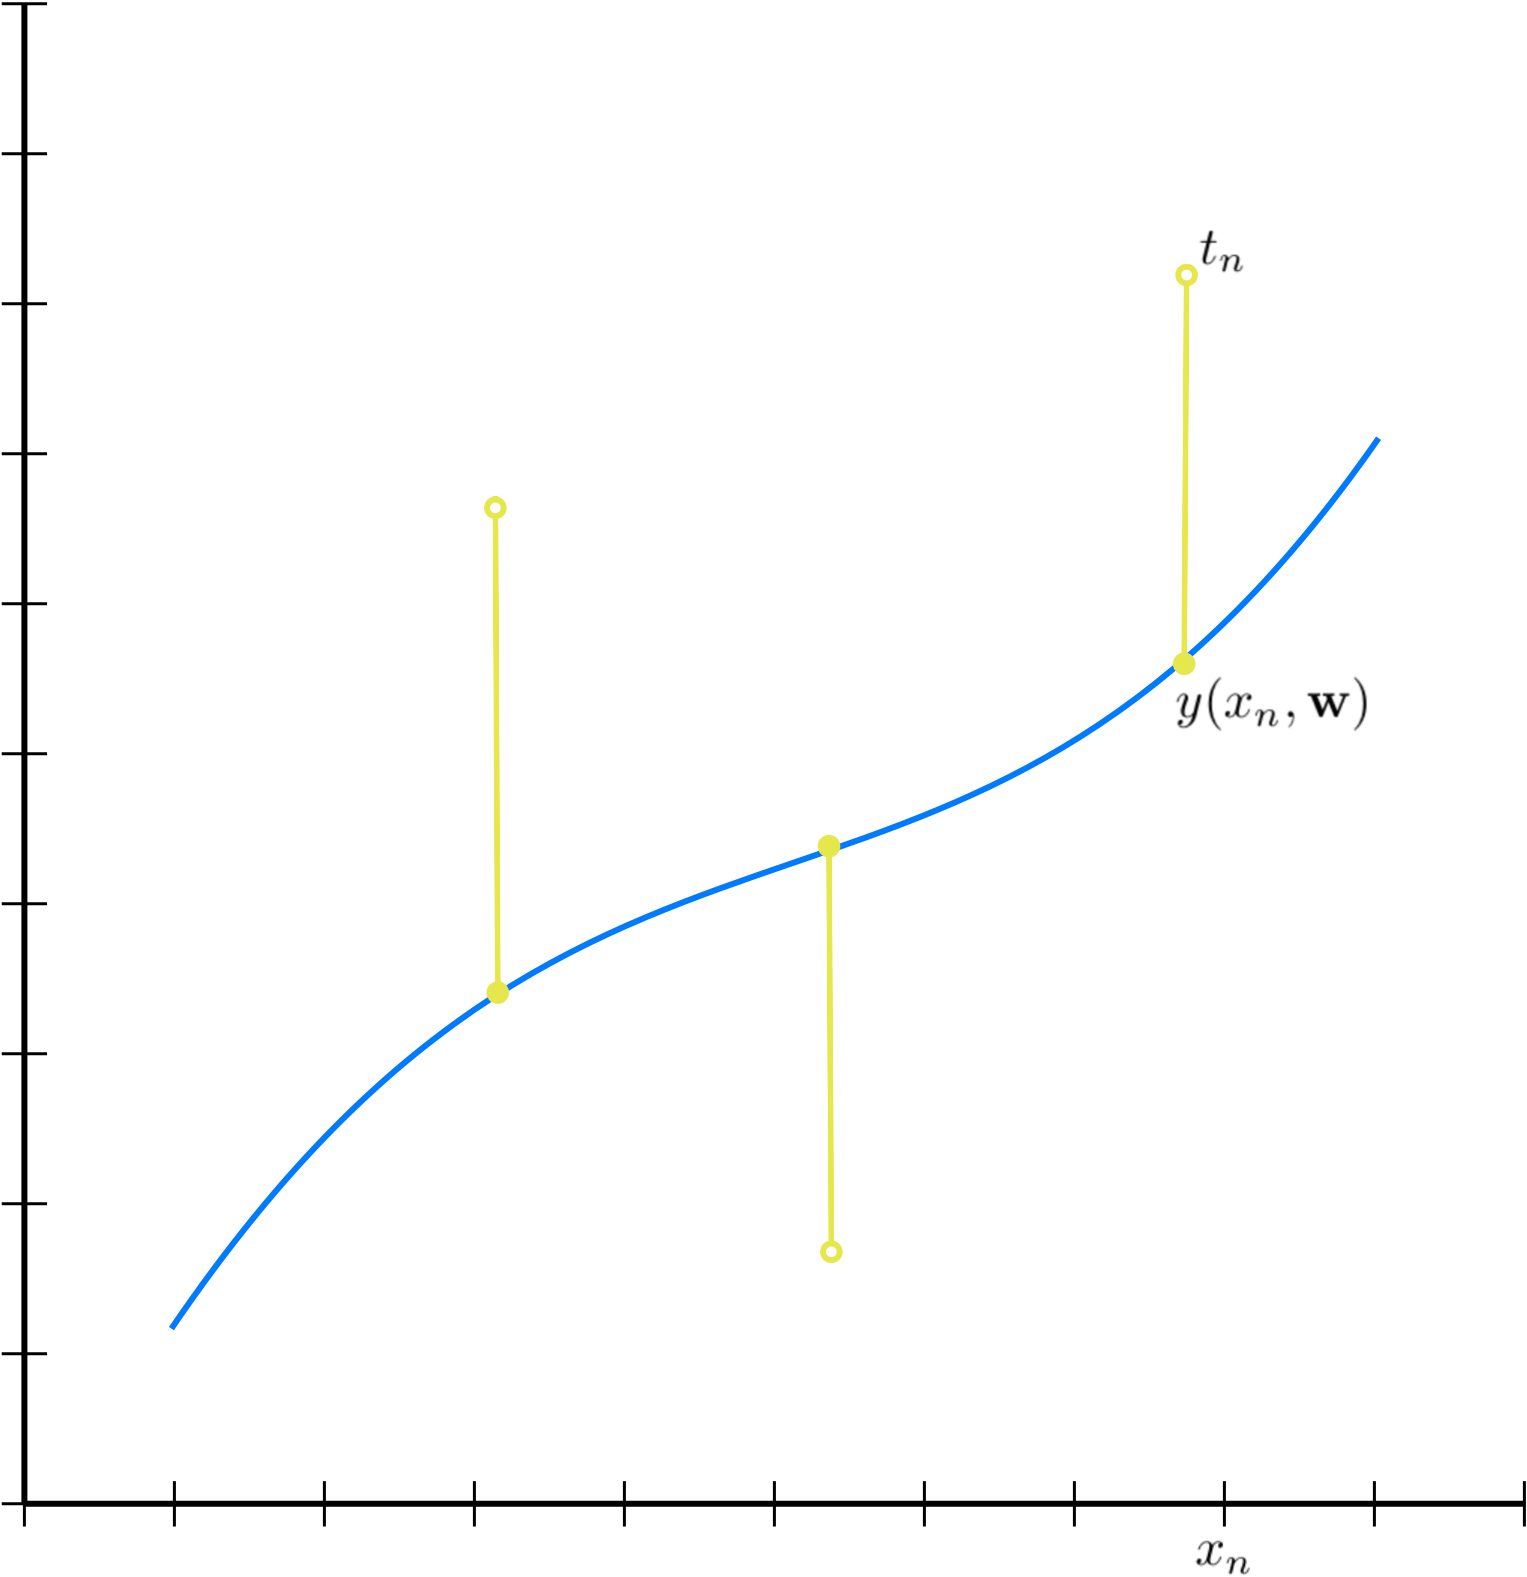
\includegraphics[width=0.3\textwidth]{"Temas/Tema 1/SSE.png"}
\end{center}

\subsection{Peligros}
\subsubsection{Subajuste y sobreajuste}

\begin{center}
	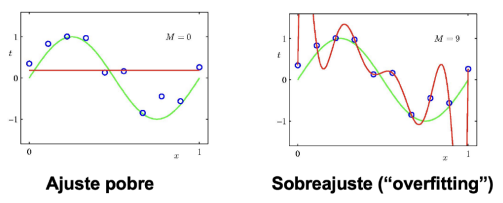
\includegraphics{"Temas/Tema 1/Ajustes.png"}
\end{center}
\subsection{Complejidad del modelo vs número de datos}
\begin{minipage}{0.6\textwidth}
	\begin{itemize}[label=\color{red}\textbullet, leftmargin=*]
		\item \color{lightblue}Comoportamiento con $M(N\text{ fijo})$
	\end{itemize}
	Fijado $N$, la complejidad del modelo determina la generalización
\end{minipage}\qquad\begin{minipage}{0.4\textwidth}
\includegraphics{"Temas/Tema 1/Screenshot001"}
\end{minipage}

\begin{minipage}{0.4\textwidth}
	\begin{itemize}[label=\color{red}\textbullet, leftmargin=*]
		\item \color{lightblue}Comportamiento con $N$ ($M$ fijo)
	\end{itemize}
	Fijado $N(M=9)$, $N$ condiciona la solución del problema: si es bajo, se puede sobreajustar, si es alto (con relación a la dimensión) se reduce el sobreajuste.
\end{minipage}